
\title{partial: An R Package for Creating Partial Dependence Plots}
\author{by Author One, Author Two and Author Three}

\maketitle

\abstract{
An abstract of less than 150 words.
}


\section{Outline}

\begin{itemize}
  \item Other packages of interest: 
  \begin{description}
    \item[\CRANpkg{plotmo}] allows for up to two variables and fixes other variables at there median values (or the first level for factors). Less accurate than partial dependence, but flexible and fast! For additive models (i.e., no interactions), these plots are identical in shape to partial dependence plots.
    \item[\CRANpkg{ICEbox}] can also calculate derivatives, but only allows for one variable at a time (i.e., no multivariate displays) -- however, color can be used to diplay information about an additional predictor.
    \item[\CRANpkg{car}] contains many functions for constructing partial-residual and marginal-model plots. The \CRANpkg{effects} is also of interest. However, these packages are orientated towards parametric models (e.g., linear and generalized linear models), whereas \pkg{plotmo}, \pkg{ICEbox}, and \pkg{partial} are mainly for nonparametric and black box models (though, they can be used for simple parametric models as well).
  \end{description}
\end{itemize}


\section{Introduction}

Predictor importance is an important task in any supervised learning problem. However, ranking variables is only part of the story and once a subset of "important" variables is identified it is often necessary to assess the relationship between them and the response. This can be done in many ways, but in machine learning it is often accomplished by constructing \dfn{partial dependence plots} (PDPs). PDPs help visualize the relationship between a subset of the predictors and the response while accounting for the average effect of the other independent variables. They are particularly effective with black box models like support vector machines or random forest.

%computing and plotting \dfn{partial dependence functions}. Partial dependence plots help visualize the relationship between a subset of the predictors and the response while accounting for the average effect of the other independent variables. They are particularly effective with \dfn{black box} models (e.g., a support vector machine or random forest).

Many techniques exist for visualizing the relationship between a predictor and the response based on a fitted model. For example, the output from complex parametric models are typically augmented with partial residual plots (see J. FOX for details). Most existing techniques arose in applied regression and typically only apply to parametric models. \dfn{Partial dependence functions} \citep{friedman-2000-greedy}, on the other hand, offer a low-dimensional graphical rendering of the prediction function $\widehat{f}\left(\boldsymbol{x}\right)$ for any type of fitted models and are especially useful in visualizing the relationships discovered by complex machine learning algorithms such as a \dfn{random forest}.

Targeted implementations of Friedman's partial dependence plots are available in packages \CRANpkg{randomForest} \citep{randomForest-pkg} and \CRANpkg{gbm}, among others. While the \pkg{randomForest} implementation will only allow for a single predictor, the \pkg{gbm} implementation can deal with any subset of the predictor space. Partial dependence functions are not restricted to tree-based models; they can be applied to any supervised learning algorithm (e.g., neural networks). However, to our knowledge, there is no general package for obtaining partial dependence plots for other types of model fits (e.g., a \dfn{conditional inference forest} as implemented by the \code{cforest} function in the \CRANpkg{party} package). The \CRANpkg{partial} package tries to close this gap by offering a general framework that can be applied to several types of fitted models -- though, package \CRANpkg{plotmo} has come a long way in this direction..

Partial dependence plots are very useful but can be misleading in the presence of substantial interactions \citep{goldstein-peeking-2015}. To overcome this issue \citet{goldstein-peeking-2015} developed the concept of \dfn{individual conditional expectation} (ICE) plots -- available in the \CRANpkg{ICEbox} package.

There are two main functions available in the \pkg{partial} package (PKG REF):
\begin{itemize}
  \item \code{partial}
  \item \code{plotPartial}
\end{itemize}
The \code{partial} function evaluates the partial dependence \eqref{eqn:pdf} from a fitted model over a grid of predctor vaulues. By default, \code{partial} returns a data frame with an dditional class: \code{"partial"}. Otherwise a \code{"lattice"} object (i.e., a plot) is returned. For more advanced plotting, the \code{plotPartial} functions will take a \code{"partial"} object and display a customizable lattice plot.

There are two ways to install the \pkg{partial} package. Obtaining the latest stable release from CRAN:
\begin{example}
install.packages("partial")
\end{example}
or installing the development version from GitHub:
\begin{example}
devtools::install_github("bgreenwell/partial")
\end{example}

\section{Partial dependence plots}

Let $\boldsymbol{x}$ represent the set of predictors in a model whose prediction function is $\widehat{f}\left(\boldsymbol{x}\right)$ (these are the values returned by \code{predict} in R). If we partition $\boldsymbol{x}$ into an interest set, $\boldsymbol{z}_s$, and its compliment, $\boldsymbol{z}_{c} = \boldsymbol{x} \setminus \boldsymbol{z}_s$, then the partial dependence of the response on $\boldsymbol{z}_s$ is defined as
\begin{equation}
\label{eqn:pdf}
\bar{f}_s\left(\boldsymbol{z}_s\right) = \frac{1}{n}\sum_{i = 1}^n\widehat{f}\left(\boldsymbol{z}_s,\boldsymbol{z}_{i, c}\right),
\end{equation}
where $\boldsymbol{z}_{i, c}$ $\left(i = 1, 2, \dots, n\right)$ are the values of $\boldsymbol{z}_c$ that occur in the training sample. This can be quite computationally intensive since Equation~\eqref{eqn:pdf} involves a pass over the training records for each set of combinations of $\boldsymbol{z}_s$. Fortunately, this problem is \dfn{embarrassingly parallel}.

The basic algorithm for computing a partial dependence function is as follows:
\begin{enumerate}
  \item Fit a model
  \item Suppose $x_i$ is the predictor set of interest. For each unique value of $x_i$, do the following:
  \begin{enumerate}
    \item Make a copy of the original training data and replace $x_i$ with the unique value -- everything else remains th same.
    \item Compute the predicted values using the modified copy of the training data.
    \item Average the predictions over each of the observations.
  \end{enumerate}
  \item Plot the average prediction against $x_i$.
  \item Repeat for each predictor of interest.
\end{enumerate}


\section{Partial dependence plots in R}

For illustration, we will use the (corrected) Boston housing data which are available from the \CRANpkg{mlbench} package. We begin by loading the data and omitting unimportant columns.
\begin{example}
data(BostonHousing2, package = "mlbench")  # load the data
boston <- BostonHousing2[, -c(1, 2, 5)]
\end{example}

Next, we fit a traditional random forest (as implemented in the \CRANpkg{randomForest} package) to the entire data set. 
\begin{example}
# Load required packages
library(partial)
library(randomForest)

# Fit a random forest
set.seed(101)  # for reproducibility
fit.rf <- randomForest(cmedv ~ ., data = boston, importance = TRUE)
print(fit.rf)  # check model results
varImpPlot(fit.rf, main = "")  # variable importance plot

# Call:
#   randomForest(formula = cmedv ~ ., data = boston, importance = TRUE) 
# Type of random forest: regression
# Number of trees: 500
# No. of variables tried at each split: 5
# 
# Mean of squared residuals: 9.114248
# % Var explained: 89.17
\end{example}
The model fit is reasonable, with an \dfn{out-of-bag} $R^2$ of 0.89. The variable importance scores are displayed in Figure~\ref{fig:plotmo_vs_partial}. Both plots indicate that the percentage of lower status of the population (\code{lstat}) and the average number of rooms per dwelling (\code{rm}) are highly associated with the median value of owner-occupied homes. The question then arises, "What is the nature of these associations?" To help answer this, we can look at the partial dependence of \code{cmedv} on \code{lstat} and \code{rm}, individually and together. 

\begin{figure}[htbp]
  \centering
  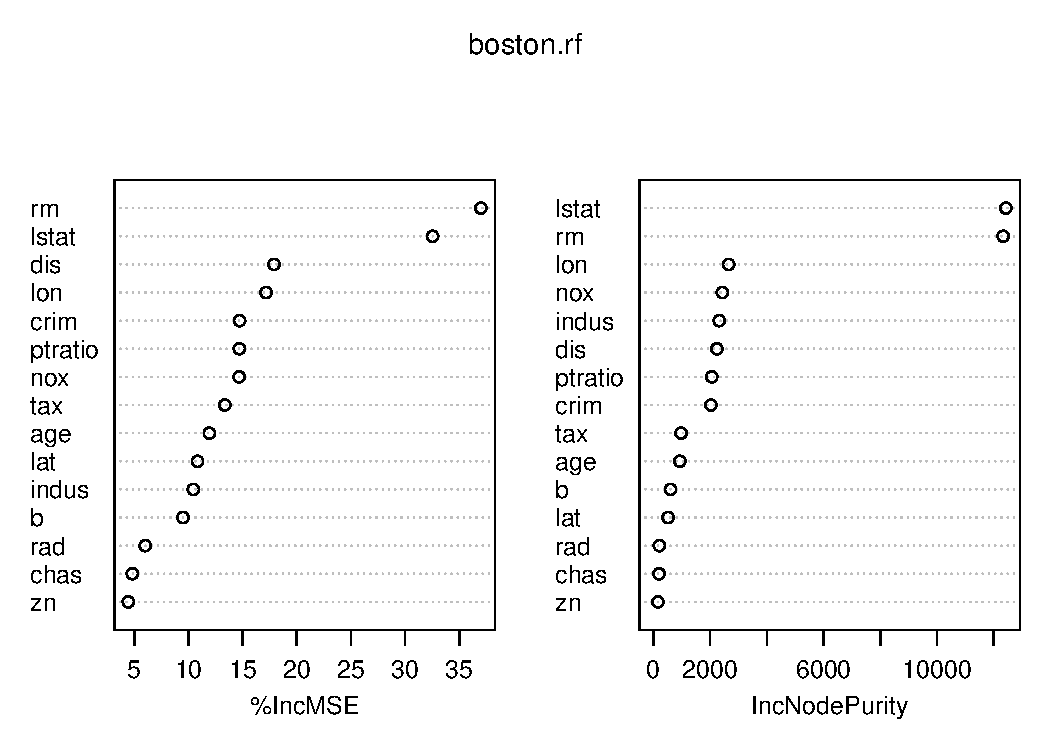
\includegraphics[width=0.8\linewidth]{boston_rf_vimp}
  \caption{Dotchart of variable importance scores for the Boston housing data based on a random forest with 500 trees.}
  \label{fig:plotmo_vs_partial}
\end{figure}

\subsection{Univariate partial dependence}

As previously mentioned, the \code{randomForest} package has its own \code{partialPlot} function for displaying partial dependence of the response on a single predictor. For example, the following snippet of code plots the partial dependence of \code{cmedv} on \code{lstat}:
\begin{example}
partialPlot(fit.rf, pred.data = boston, x.var = "lstat")
\end{example}
The same plot (implemented in \pkg{lattice}) can be achieved using the \code{partial} function and setting \code{plot = TRUE} (the default is \code{FALSE}):
\begin{example}
partial(fit.rf, pred.var = "lstat", plot = TRUE)
\end{example}
\begin{figure}[htbp]
  \centering
  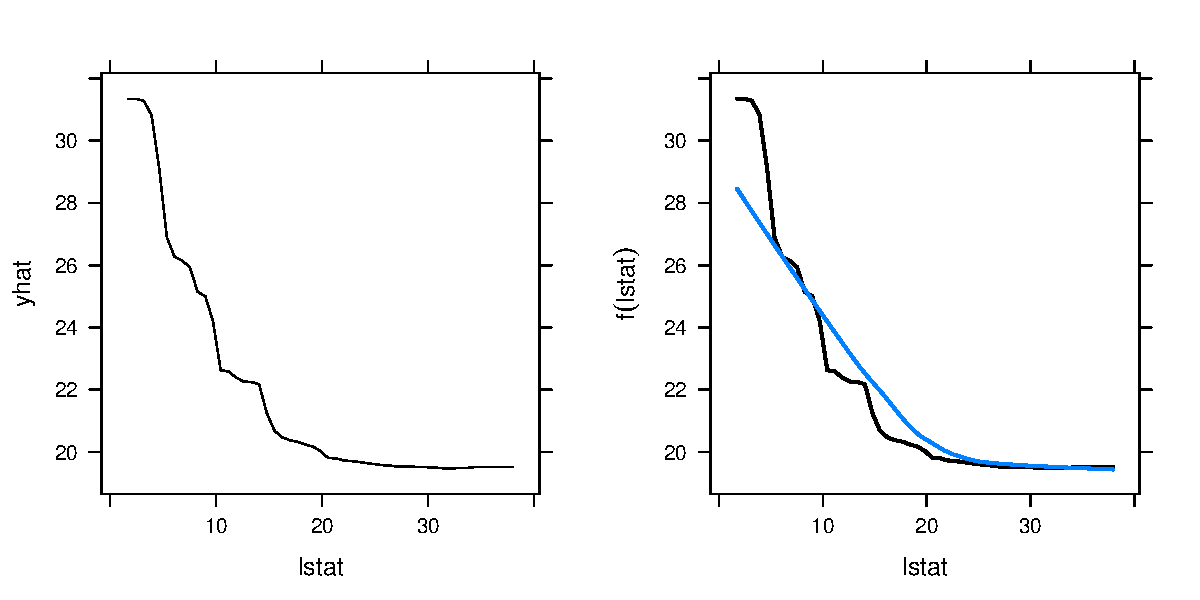
\includegraphics[width=0.8\linewidth]{pd_lstat}
  \caption{Partial dependence of \code{cmedv} on \code{lstat}.}
  \label{fig:pd_lstat}
\end{figure}

By default, \code{partial} returns a data frame:
\begin{example}
head(partial(fit.rf, pred.var = "lstat"))

#    lstat        y
# 1 1.7300 31.34696
# 2 2.4548 31.34564
# 3 3.1796 31.28286
# 4 3.9044 30.82356
# 5 4.6292 29.12636
# 6 5.3540 26.89093
\end{example}


The benefit of using \code{partial} is threefold: (1) it is a generic function that can be used for other types of model fits (e.g., a \dfn{conditional inference forest} as implemented in the \CRANpkg{party} package), (2) it will allow for any number of predictors to be used, and (3) it can utilize any of the parallel backends supported by the \CRANpkg{foreach} package (more on this later). For example, to assess the joint effect of \code{lstat} and \code{rm} on \code{cmedv} we could use
\begin{example}
partial(fit.rf, pred.var = c("lstat", "rm"), plot = TRUE)
\end{example}

Finer plotting control can be achieved using the accompanying \code{plotPartial} function. \code{plotPartial} takes a \code{"partial"} object and provides a convenient \CRANpkg{lattice} display that can be easily tailored. For example, the code chunk
\begin{example}
pd.lstat.rm <- partial(fit.rf, pred.var = c("lstat", "rm"))
p1 <- plotPartial(pd.lstat.rm)
p2 <- plotPartial(pd.lstat.rm, contour = FALSE, zlab = "cmedv", drape = TRUE, 
                  colorkey = TRUE, screen = list(z = -20, x = -60))
print(p1, position = c(0, 0, 0.5, 1), more = TRUE)
print(p2, position = c(0.5, 0, 1, 1))
\end{example}
produces the three-dimensional displays in Figure~\ref{fig:pd_lstat_rm}.
\begin{figure}[htbp]
  \centering
  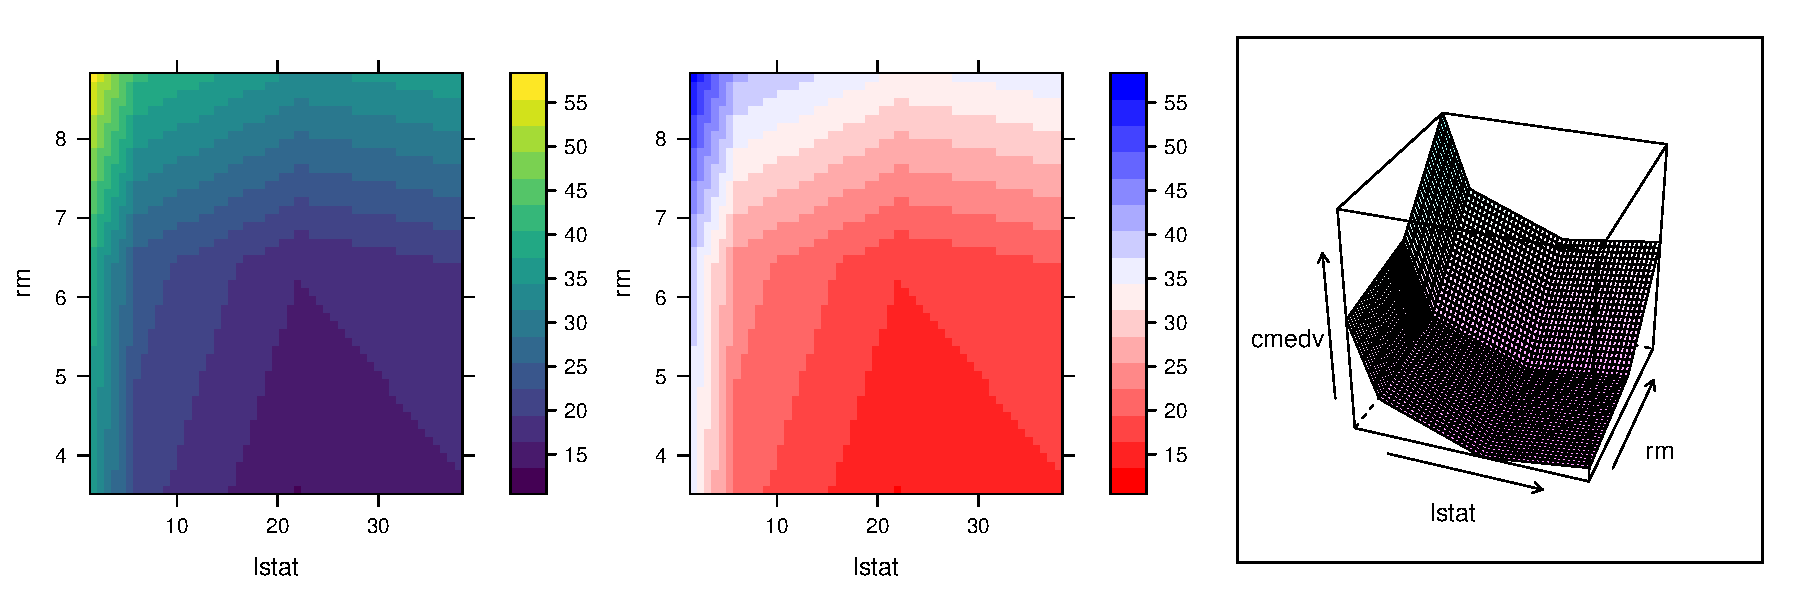
\includegraphics[width=1.0\linewidth]{pd_lstat_rm}
  \caption{Partial dependence of \code{cmedv} on \code{lstat} and \code{rm}.}
  \label{fig:pd_lstat_rm}
\end{figure}

Unfortunately, the \code{cforest} implementation contains no such function. In this case we can use \code{partial}:
\begin{example}
crf.lstat <- partial_1d(fit.crf, x.name = "lstat", n = 51)
crf.rm <- partial_1d(fit.crf, x.name = "rm", n = 51)
par(mfrow = c(1, 2))
plot(crf.lstat, type = "l")
plot(crf.rm, type = "l")
\end{example}

In some cases it is difficult for \code{partial} to tell whether the response is continuous (regression) or categorical (classification). For these cases, we added the option \code{super.type} which accepts a character string specifying either \code{"regression"} or \code{"classification"} -- this distinction is important because for classification problems, PDPs use something similar to a \dfn{logit} scale for response estimation.

By default \code{partial} returns a data frame. If called with \code{plot = TRUE}, however, a lattice plot is displayed instead
\begin{example}
partial_1d(fit.crf, x.name = "lstat", n = 51, plot = TRUE)
\end{example}

\subsection{Multivariate partial dependence}

Bivariate (and higher order) partial dependence can also be handled

\begin{example}
# Bivariate partial dependence
rf.rm.lstat <- partial_2d(fit.rf, x1.name = "rm", x2.name = "lstat", 
                          n1 = 51, n2 = 51, .progress = "text")
wireframe(y ~ rm * lstat, data = rf.rm.lstat, zlab = "cmedv", drape = TRUE, 
          colorkey = TRUE, screen = list(z = 110, x = -60))
\end{example}

The variables are plotted in the order they are given; that is, the first variable is plotted along the $x$-axis, the second on the $y$-axis, and the rest becom panel variables. Hence, it is best to use numeric variables for the first two, and factors for the remaining. The following snippet of code plots the partial dependence of \code{cmedv} on \code{rm}, \code{lstat}, and \code{chas}, but since \code{chas} is a binary variable (whether or not the census tract bounds river), a separate panel is displayed for each category.
\begin{example}
# Trivariate partial dependence
rf.rm.lstat.ptratio <- partial_3d(fit.rf, x1.name = "rm", x2.name = "lstat", 
                                  x3.name = "chas", n1 = 51, n2 = 51, n2 = 51, 
                                  .progress = "text")
wireframe(y ~ rm * lstat, data = rf.rm.lstat, zlab = "cmedv", drape = TRUE, 
          colorkey = TRUE, screen = list(z = 110, x = -60))
\end{example}

\subsection{The Boston Housing Data}

In \pkg{plotmo} the other variables are held fixed at their median values. This results in a less accurate, but much faster display. To illustrate we fit a multivariate adaptive regression spline (MARS) model to the Boston housing data. MARS models can be fit using the \code{mars} function from the \CRANpkg{mda} package, or using the \code{earth} function from the \CRANpkg{earth} package. Here we use the \pkg{earth} implementation which conveniently loads the \pkg{plotmo} package as well.
\begin{example}
# Fit a MARS model
fit.earth <- earth(cmedv ~ ., data = boston, degree = 3)

# Partial dependence function
earth.rm <- partial_1d(fit.earth, x.name = "rm")

# Compare partial and plotmo
pdf("plotmo_vs_partial.pdf", width = 7, height = 5)
plotmo(fit.earth, degree1 = "rm", degree2 = FALSE, do.par = FALSE, 
       ylim = c(16.79417, 41.87501), main = "", xlab = "rm", ylab = "cmedv")
lines(earth.rm, lty = 2)
legend("topleft", legend = c("plotmo", "partial"),
       lty = 1:2, inset = 0.01)
dev.off()
\end{example}

\begin{figure}[htbp]
  \centering
  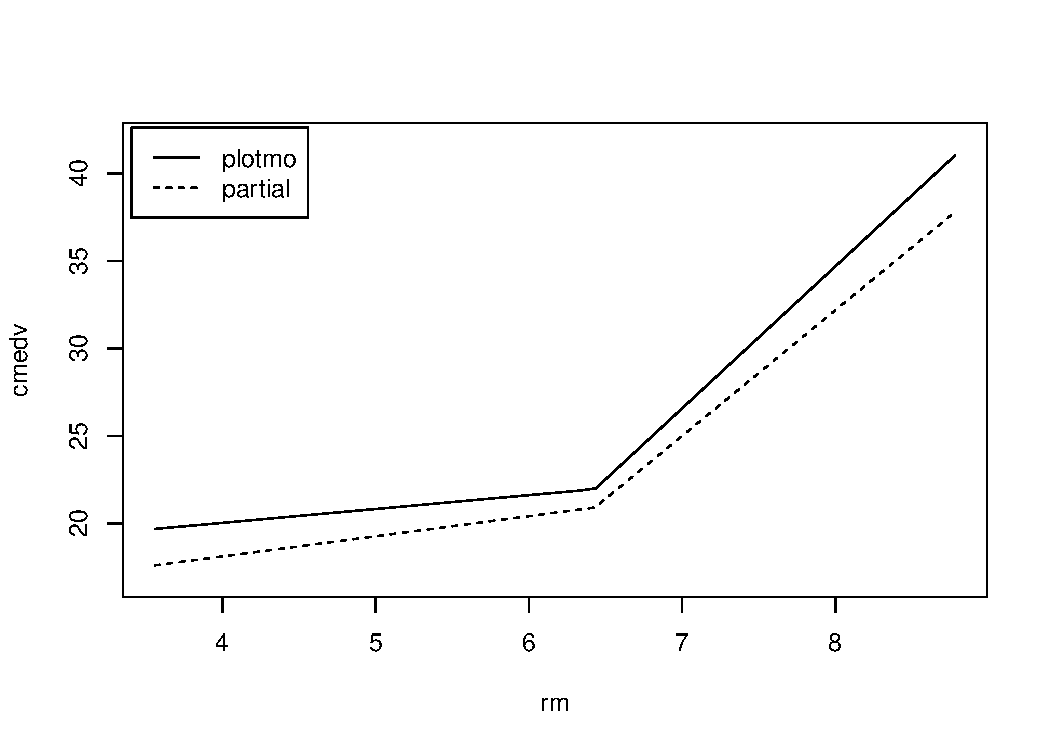
\includegraphics[width=0.8\linewidth]{plotmo_vs_partial}
  \caption{The logo of R.}
  \label{figure:plotmo_vs_partial}
\end{figure}

\begin{example}
partial(fit.earth, pred.var = c("rm", "ptratio"), plot = TRUE)
\end{example}

\begin{figure}[htbp]
  \centering
  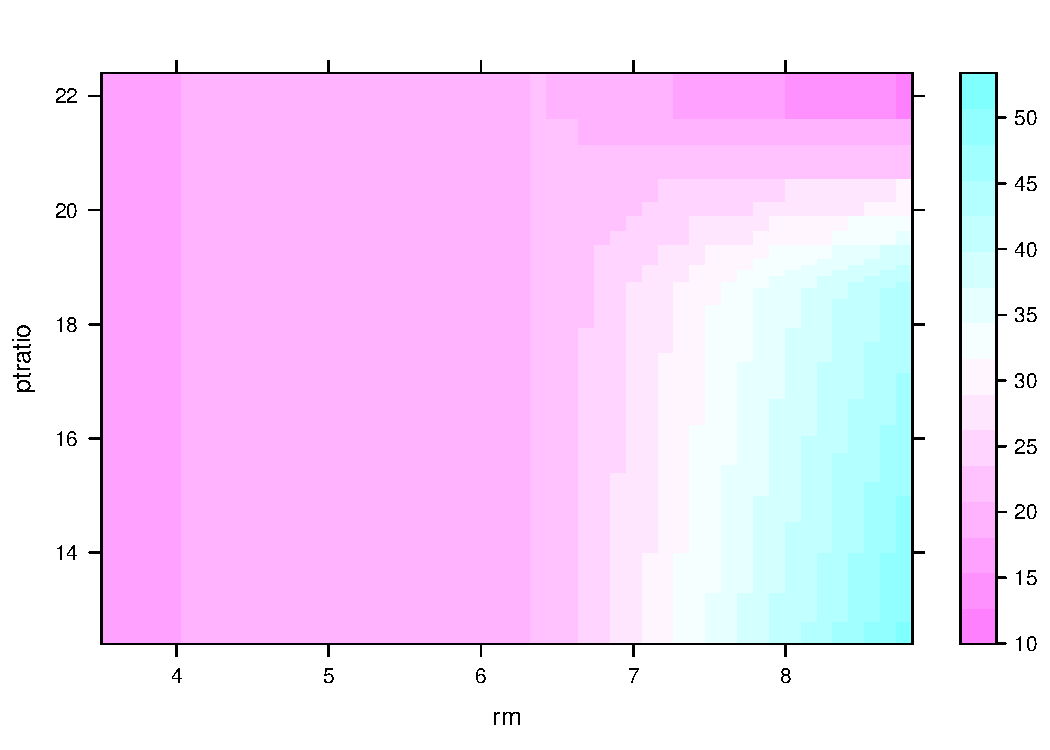
\includegraphics[width=0.8\linewidth]{earth_rm_ptratio}
  \caption{Partial dependence of \code{cmedv} on \code{rm} and \code{ptratio}.}
  \label{figure:earth_rm_ptratio}
\end{figure}

\code{partial} returns a\code{"data.frame"} object with an additioanl class called \code{"partial"}; the additional class is recognized by \code{plotPartial} for convenient default plotting. To create more elaborate plots, just work with the data frame directly. Also, the convenient \code{plot} option in \code{partial} returns a basic plot, but is not as customizable as uning plotPartial. The following snipet of code demonstrates:
\begin{example}
# Basic partial dependence plot
partial(fit.rf, "rm", plot = TRUE)

# Save the partial dependence data for customized plotting
pd.rm <- partial(fit.rf, "rm")
partialPlot(pd.rm, xlab = "Average number of rooms", ylab = "Median home value")
plot(pd.rm, type = "l")  # base R graphics

# Try using ggplot2
library(ggplot2)
ggplot(pd.rm, aes(rm, y)) +
  geom_point() +
  geom_line() +
  theme_light()
\end{example}

\subsection{Avoiding extrapolation}

There are few ways to mitigate the risk of extrapolation in PDPs: rug displays and convex hulls. Rug displays are one-dimensional plots added to the axes. The \code{plotPartial} has a \code{rug} option that will display the deciles of the distribution  (as well as the minimum and maximum values) for the predictors on the horizontal or vertical axes. The following snippet of code produces the plot on the left side of Figure~\ref{fig:partial_extrap}. Notice that in both examples we had to provide the original training data to \code{plotPartial} via the \code{training.data} option.
\begin{example}
plotPartial(pf.lstat, rug = TRUE, training.data = boston)
\end{example}

In higher dimensions, plotting the convex hull is more informative; it outlines the region of the predictor space that the model was trained on. When \code{convex.hull = TRUE}, the convex hull of the first two dimensions of $\boldsymbol{z}_s$ (i.e., the variables used for the horizontal and vertical axes) is added to the plot. Over interpreting the partial dependence plot outside of this region can be dangerous. The right side of Figure~\ref{fig:partial_extrap} was produced using:
\begin{example}
plotPartial(pd.lstat.rm, convex.hull = TRUE, training.data = boston)
\end{example}

\begin{figure}[htbp]
  \centering
  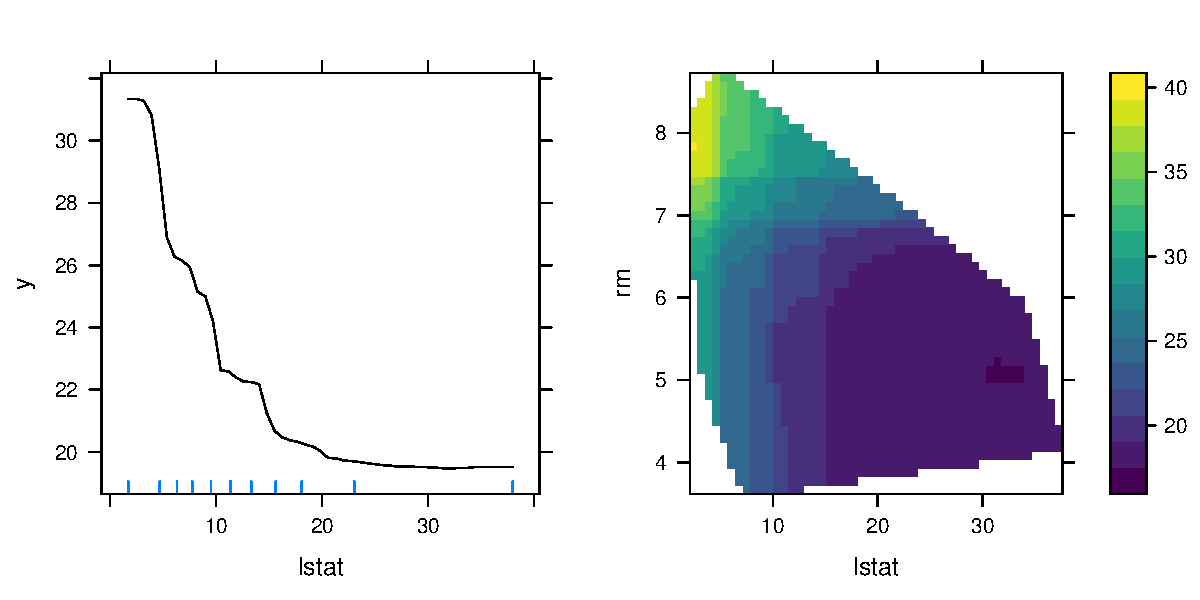
\includegraphics[width=0.8\linewidth]{partial_extrap}
  \caption{Examples of partial dependence plots with the addition of a rug display (left) and a convex hull (right).}
  \label{fig:partial_extrap}
\end{figure}

\subsection{Addressing computational concerns}

Additional options are available to ease the computational intensity for large problems. For example, there was no need to compute partial dependence of median home value using each uniqe value of \code{rm} in the training data (which would require 446 passes over the data!). We could get very reasonable results using a reduced number of points. Current options are to use a grid of equally spaced values in the range of the variable of interest; the number of points is controlled by the option \code{n.pts}. Alternatively, a specific set of values can be supplied (e.g., quantiles of interest) through the \code{pred.data} argument. For example, the following snippet of code re-computes the partial dependence of median home value on \code{rm} using both options; the results are displayed in Figure~\ref{fig:partial_manual}.
\begin{example}
partial(fit.rf, "rm", grid.resolution = 30, plot = TRUE)
partial(fit.rf, "rm", pred.grid = 3:9, plot = TRUE)
\end{example}

\begin{figure}[htbp]
  \centering
  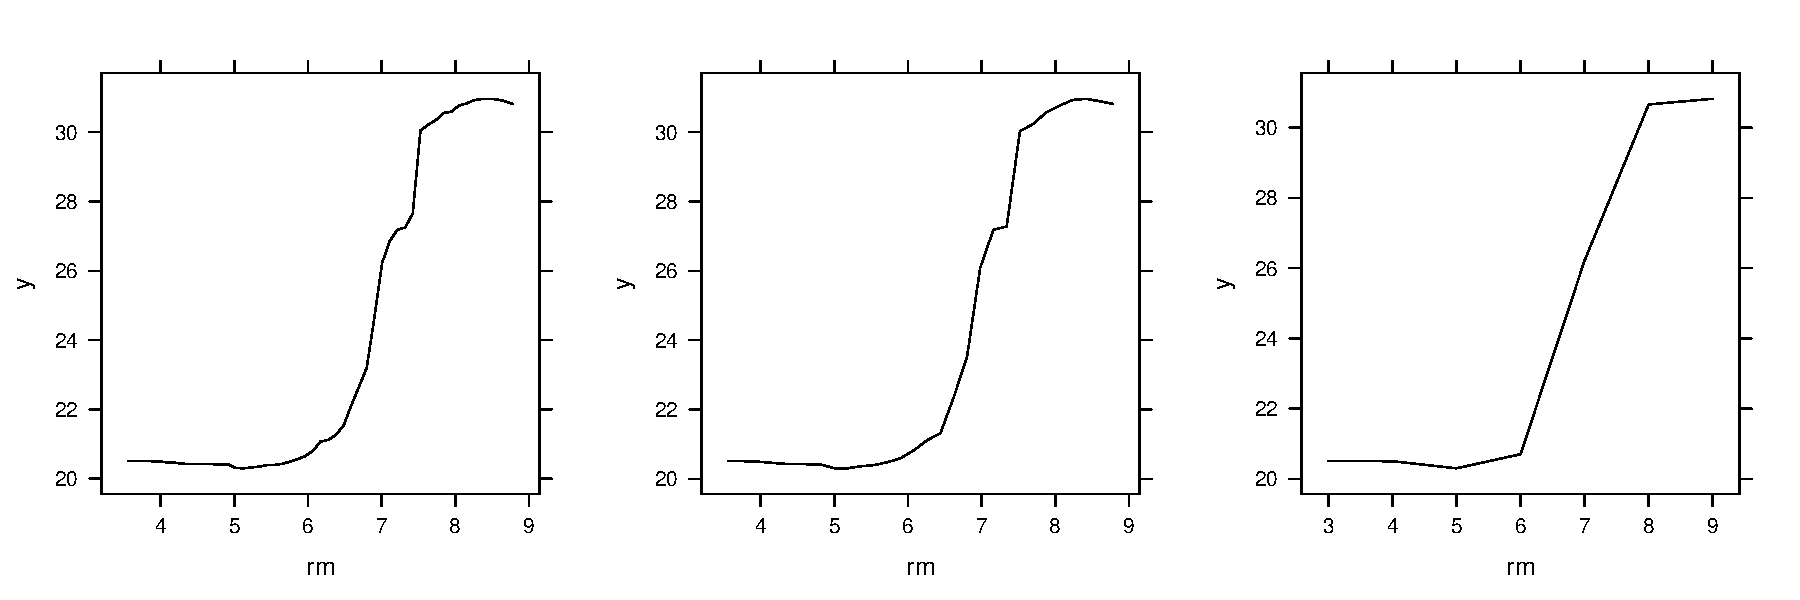
\includegraphics[width=0.8\linewidth]{partial_manual}
  \caption{Examples of partial dependence plots using a reduced set of predictor values.}
  \label{fig:partial_manual}
\end{figure}

The \code{partial} function relies on the \CRANpkg{plyr} package \citep{plyr-pkg}, rather than for loops. This makes it poosible to request progress bars (e.g., \code{.progress = "text"}) or run \code{partial} in parallel. In fact, \code{partial} can use any of the parallel backends supported by the \CRANpkg{foreach} package. To use this functionality, we must load and register a supported parallel backend (e.g., \CRANpkg{doParallel} or \CRANpkg{doMC}). The following snippet of code obtains the partial dependence of median home value on \code{rm}, \code{lstat}, and \code{ptratio} in parallel. The result is displayed in Figure~\ref{fig:partial_3}.
\begin{example}
library(doParallel)
cl <- makeCluster(2)  # using snow-like functionality
registerDoParallel(cl)  # use cores = 2 for multicore functionality
pd3 <- partial(fit.rf, pred.var = c("lstat", "rm", "ptratio"),
               grid.resolution = 10, .parallel = TRUE)
stopCluster(cl)  # required when using snow-like functionality
plotPartial(pd3, number = 4, overlap = 0.1)
\end{example}

\begin{figure}[htbp]
  \centering
  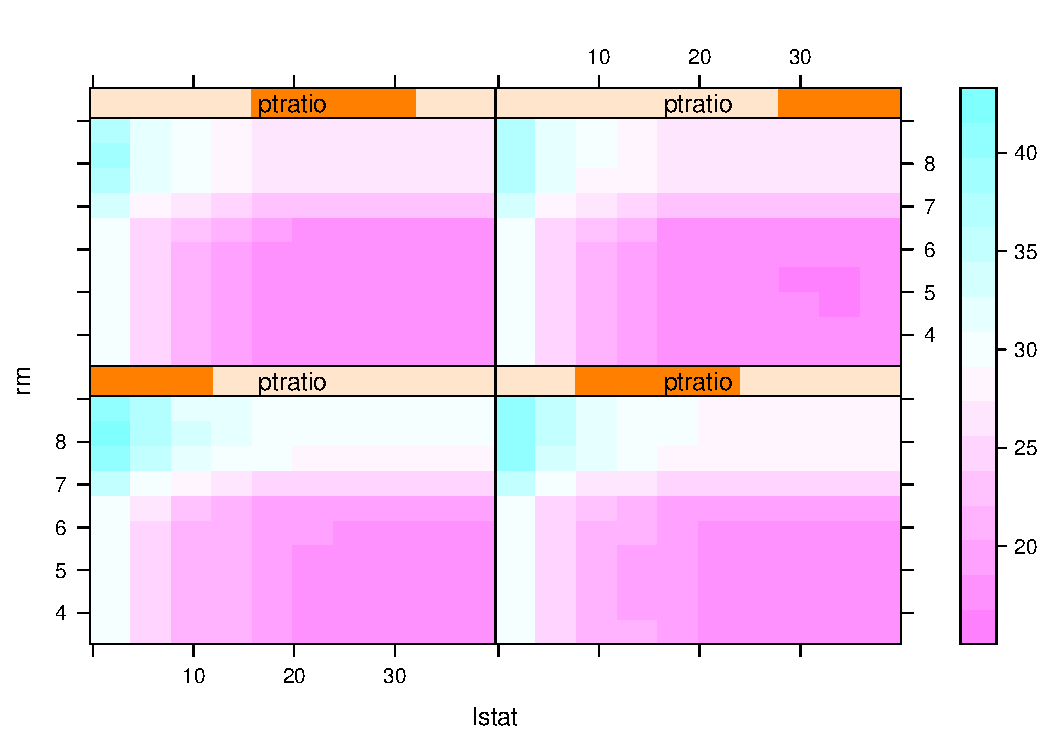
\includegraphics[width=0.8\linewidth]{partial_3}
  \caption{Examples of partial dependence plots using a reduced set of predictor values.}
  \label{fig:partial_3}
\end{figure}

\subsection{Classification problems}

For classification problems, partial dependence functions are on a scale simliar to the logit; in particular, an average logit. Suppose the response is categorical with $K$ levels, then for each class we have
\begin{equation}
\label{eqn:avg-logit}
f_k(x) = \log\left[p_k(x)\right] - \frac{1}{K}\sum_{i = 1}^K\log\left[p_k(x)\right], \quad k = 1, 2, \dots, K,
\end{equation}
where $p_k(x)$ is the predicted probability for the $k$-th class. Plotting $f_k(x)$ helps us understand how the log-odds for the $k$-th cass depends on different subsets of the predictor variables.

To illustrate, consider the Edgar Anderson's iris data from the \CRANpkg{datasets} package. We fit a support vector machine with a radial basis function kernel to the data (the parameters were determined using 5-fold cross-validation).
\begin{example}
library(kernlab)
iris.svm <- ksvm(Species ~ ., data = iris, kernel = "rbfdot", C = 0.25,
                 kpar = list(sigma = 0.75), prob.model = TRUE)
\end{example}

Next, we plot the partial dependence of \code{Species} on both \code{Petal.Width} and \code{Petal.Length} for each of the three classes. The result is displayed in Figure~\ref{fig:partial_iris}.
\begin{example}
pd <- NULL
for (i in 1:3) {
  tmp <- partial(iris.svm, pred.var = c("Petal.Width", "Petal.Length"), 
                 which.class = i, training.data = iris)
  pd <- rbind(pd, cbind(tmp, Species = levels(iris$Species)[i]))
}
levelplot(y ~ Petal.Width * Petal.Length | Species, data = pd)
\end{example}

\begin{figure}[htbp]
  \centering
  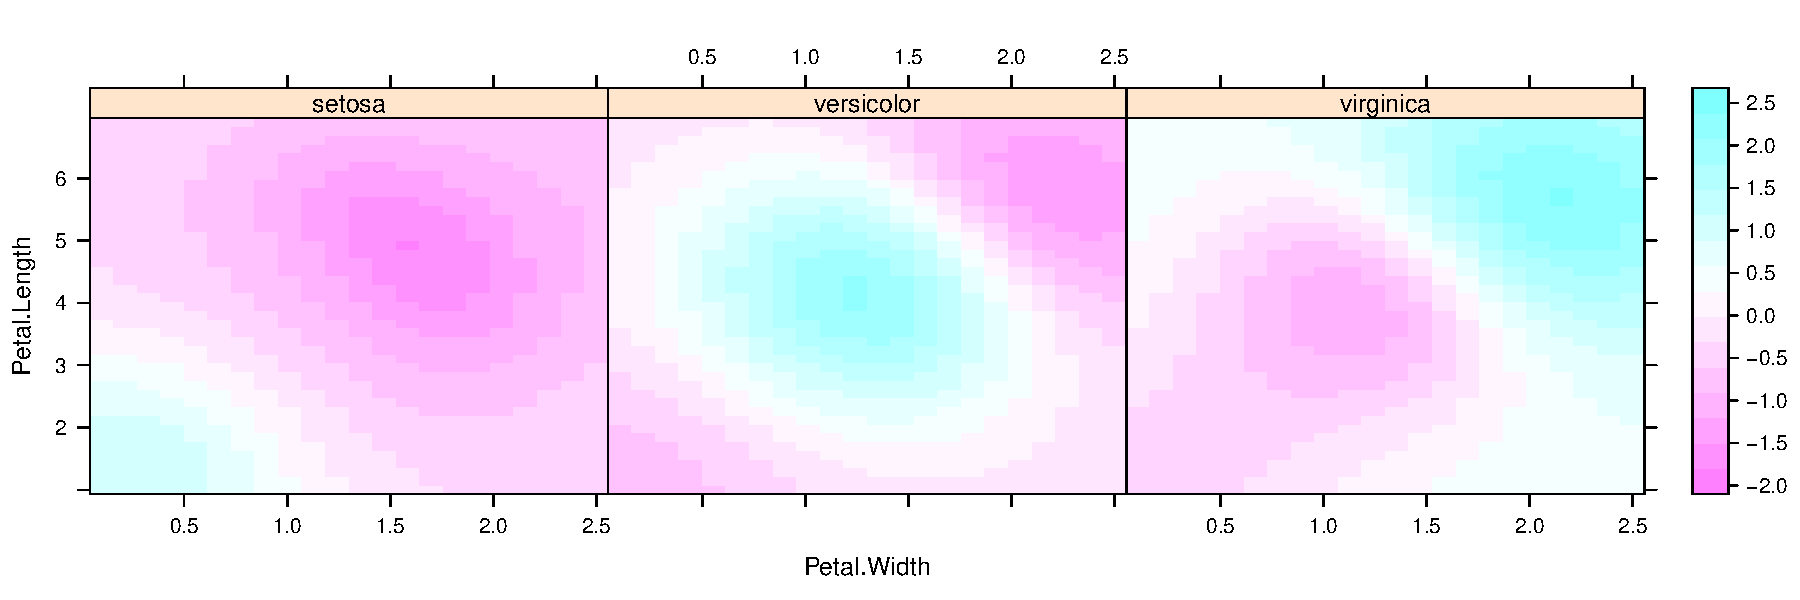
\includegraphics[width=1.0\linewidth]{partial_iris}
  \caption{Partial dependence of species on petal width and petal length for the iris data.}
  \label{fig:partial_iris}
\end{figure}

\section{Summary}

In the future, this package will be expanded to appropriately handle other types of responses as well (e.g., countd data).

\bibliography{Greenwell}

\address{Brandon Greenwell\\
  Infoscitex, a dcs company\\
  4027 Colonel Glenn Highway\\
  Suite 210\\
  Dayton, OH 45431-1672\\
  United States of America\\}
\email{bgreenwell@infoscitex.com}
 